%%%%%%%%%%%%%%%%%%%%%%%%%%%%%%%%%%%%%%%%%
% Document Author: Plinio H. Vargas
% Course: CS-532, Spring 2016 at Old Dominion University
%
% Structured General Purpose Assignment
% LaTeX Template
%
% This template has been downloaded from:
% http://www.latextemplates.com
%
% Original template author:
% Ted Pavlic (http://www.tedpavlic.com)
%
% Note:
% The \lipsum[#] commands throughout this template generate dummy text
% to fill the template out. These commands should all be removed when 
% writing assignment content.
%
%%%%%%%%%%%%%%%%%%%%%%%%%%%%%%%%%%%%%%%%%
%----------------------------------------------------------------------------------------
%	PACKAGES AND OTHER DOCUMENT CONFIGURATIONS
%----------------------------------------------------------------------------------------

\documentclass{article}

\usepackage{fancyhdr} % Required for custom headers
\usepackage{lastpage} % Required to determine the last page for the footer
\usepackage{extramarks} % Required for headers and footers
\usepackage{listings}
\usepackage{graphicx} % Required to insert images
\usepackage{lipsum} % Used for inserting dummy 'Lorem ipsum' text into the template
\usepackage[bookmarks,bookmarksopen,bookmarksdepth=2]{hyperref} % for bookmarks
\usepackage{enumerate}
\usepackage{csquotes} % for quoting things
\usepackage{multirow}
\usepackage{amsmath}
\usepackage{navigator}
\usepackage{caption}
\usepackage[shortlabels]{enumitem}
\usepackage{lmodern}
\usepackage[utf8]{inputenc}
%\usepackage[table]{xcolor}% http://ctan.org/pkg/xcolo
\usepackage[dvipsnames]{xcolor}
\usepackage{longtable}
\usepackage{textcomp}
\usepackage{url}
\usepackage{import}
\usepackage{float}
\usepackage{dashrule} % for dashline
\usepackage{keystroke}

\lstdefinestyle{numbers}
{ frame=tb,
  language=python,
  aboveskip=3mm,
  belowskip=3mm,
  showstringspaces=false,
  columns=flexible,
  basicstyle={\small\ttfamily},
  numbers=left,
  numberstyle=\tiny\color{gray},
  keywordstyle=\color{blue},
  commentstyle=\color{OliveGreen},
  stringstyle=\color{purple},
  breaklines=true,
  breakatwhitespace=true,
  tabsize=3
}

\lstdefinestyle{nonumbers}
{ frame=shadowbox,
  language=python,
  aboveskip=3mm,
  belowskip=3mm,
  showstringspaces=false,
  columns=flexible,
  basicstyle={\small\ttfamily},
  numbers=none,
  numberstyle=\tiny\color{gray},
  keywordstyle=\color{blue},
  commentstyle=\color{OliveGreen},
  stringstyle=\color{purple},
  breaklines=true,
  breakatwhitespace=true,
  tabsize=3
}

\lstdefinestyle{mybox}
{
	basicstyle={\small\ttfamily},
    numbers=left,
    numberstyle=\tiny\color{gray},
    stepnumber=1,
    numbersep=5pt,
    showspaces=false, % don't show spaces by adding underscores
    showstringspaces=false, % don't underline spaces in strings
    showtabs=false, % don't show tabs with underscores
    frame=shadowbox,
    tabsize=4,
    captionpos=b,
    breaklines=true,
    breakatwhitespace=false,
  	keywordstyle=\color{blue},
	commentstyle=\color{OliveGreen},
  	stringstyle=\color{purple},    
    rulesepcolor=\color{red!20!green!20!blue!20},
    numberbychapter=false,
    stringstyle=\color{purple},
}
% Margins
\topmargin=-0.45in
\evensidemargin=0in
\oddsidemargin=0in
\textwidth=6.5in
\textheight=9.0in
\headsep=0.25in 

\linespread{1.1} % Line spacing
\newcommand*{\medtau}{\mathbin{\scalebox{1.5}{$\tau$}}}% increase size of tau
\newcommand*{\medtaub}{\mathbin{\scalebox{1.5}{$\tau_b$}}}% increase size of tau_b
\newcommand\multibrace[3]{\rdelim\}{#1}{3mm}[\pbox{#2}{#3}]}

% Set up the header and footer
\pagestyle{fancy}
\lhead{\hmwkAuthorName} % Top left header
\chead{\hmwkShortClass\ (\hmwkClassInstructor\ \hmwkClassTime): \hmwkShortTitle} % Top center header
%\rhead{\firstxmark} % Top right header
\rhead{} % Top right header
\lfoot{\lastxmark} % Bottom left footer
\cfoot{} % Bottom center footer
\rfoot{Page\ \thepage\ of\ \pageref{LastPage}} % Bottom right footer
\renewcommand\headrulewidth{0.4pt} % Size of the header rule
\renewcommand\footrulewidth{0.4pt} % Size of the footer rule

\setlength\parindent{0pt} % Removes all indentation from paragraphs

%----------------------------------------------------------------------------------------
%	DOCUMENT STRUCTURE COMMANDS
%	Skip this unless you know what you're doing
%----------------------------------------------------------------------------------------

% Header and footer for when a page split occurs within a problem environment
\newcommand{\enterProblemHeader}[1]{
\nobreak\extramarks{#1}{#1 continued on next page\ldots}\nobreak
\nobreak\extramarks{#1 (continued)}{#1 continued on next page\ldots}\nobreak
}

% Header and footer for when a page split occurs between problem environments
\newcommand{\exitProblemHeader}[1]{
\nobreak\extramarks{#1 (continued)}{#1 continued on next page\ldots}\nobreak
\nobreak\extramarks{#1}{}\nobreak
}

\setcounter{secnumdepth}{0} % Removes default section numbers
\newcounter{homeworkProblemCounter} % Creates a counter to keep track of the number of problems

\newcommand{\homeworkProblemName}{}
\newenvironment{homeworkProblem}[1][Problem \arabic{homeworkProblemCounter}]{ % Makes a new environment called homeworkProblem which takes 1 argument (custom name) but the default is "Problem #"
\stepcounter{homeworkProblemCounter} % Increase counter for number of problems
\renewcommand{\homeworkProblemName}{#1} % Assign \homeworkProblemName the name of the problem
\section{\homeworkProblemName} % Make a section in the document with the custom problem count
\enterProblemHeader{\homeworkProblemName} % Header and footer within the environment
}{
\exitProblemHeader{\homeworkProblemName} % Header and footer after the environment
}

\newcommand{\problemAnswer}[1]{ % Defines the problem answer command with the content as the only argument
\noindent\framebox[\columnwidth][c]{\begin{minipage}{0.98\columnwidth}#1\end{minipage}} % Makes the box around the problem answer and puts the content inside
}

\newcommand{\homeworkSectionName}{}
\newenvironment{homeworkSection}[1]{ % New environment for sections within homework problems, takes 1 argument - the name of the section
\renewcommand{\homeworkSectionName}{#1} % Assign \homeworkSectionName to the name of the section from the environment argument
\subsection{\homeworkSectionName} % Make a subsection with the custom name of the subsection
\enterProblemHeader{\homeworkProblemName\ [\homeworkSectionName]} % Header and footer within the environment
}{
\enterProblemHeader{\homeworkProblemName} % Header and footer after the environment
}
   
%----------------------------------------------------------------------------------------
%	NAME AND CLASS SECTION
%----------------------------------------------------------------------------------------

\newcommand{\hmwkTitle}{\\Assignment\ \#4: \\The \enquote{Friendship Paradox}} % Assignment title
\newcommand{\hmwkShortTitle}{Assignment 4} % Assignment title
\newcommand{\hmwkDueDate}{Thursday,\ February 25,\ 2016} % Due date
\newcommand{\hmwkClass}{CS-432/532 Introduction to Web Science} % Course/class
\newcommand{\hmwkShortClass}{CS-432/532 Web Science} % Course/class
\newcommand{\hmwkClassTime}{- Spring 2016} % Class/lecture time
\newcommand{\hmwkClassInstructor}{Dr.  Michael L. Nelson} % Teacher/lecturer
\newcommand{\hmwkAuthorName}{Plinio Vargas} % Your name
\newcommand{\hmwkAuthorEmail}{pvargas@cs.odu.edu} % Your name
%------------------------------------------------------------
% Algorithm declaration
%------------------------------------------------------------
\lstnewenvironment{algorithm}[1][] %defines the algorithm listing environment
{   
    %\refstepcounter{nalg} %increments algorithm number
    \captionsetup{labelsep=colon} %defines the caption setup for: it ises label format as the declared caption label above and makes label and caption text to be separated by a ':'
    \lstset{ %this is the stype
        frame=tB,
        numbers=left, 
        mathescape=true,
        numberstyle=\tiny,
        basicstyle={\small\ttfamily}, 
        keywordstyle=\color{blue}\bfseries\em,
        keywords={,input, output, return, 
                   datatype, function, in, 
                   if, else, for, foreach, 
                   while, write, begin, end, 
        } %add the keywords you want, or load a language as Rubens explains in his comment above.
        numbers=left,
        xleftmargin=.04\textwidth,
        #1 % this is to add specific settings to an usage of this environment (for instnce, the caption and referable label)
    }
}
{}
%----------------------------------------------------------------------------------------
%	TITLE PAGE
%----------------------------------------------------------------------------------------

\title{
\vspace{2in}
\textmd{\textbf{\hmwkClass:\ \hmwkTitle}}\\
\normalsize\vspace{0.1in}\small{Due\ on\ \hmwkDueDate}\\
\vspace{0.1in}\large{\textit{\hmwkClassInstructor\ }}
\vspace{3in}
}

\author{\textbf{\hmwkAuthorName} \\ \hmwkAuthorEmail}
\date{} % Insert date here if you want it to appear below your name

%----------------------------------------------------------------------------------------
%	EMBEDDED FILE
%----------------------------------------------------------------------------------------
\embeddedfile{facebook}{../facebook.R}
\embeddedfile{linkedin}{../linkedin.R}
\embeddedfile{twitter}{../twitter.R}
\embeddedfile{twitter2}{../twitter2.R}
\embeddedfile{Following}{../GetFollowing.py}
\embeddedfile{Friends}{../GetFriends.py}
%----------------------------------------------------------------------------------------
%	START OF DOCUMENT
%----------------------------------------------------------------------------------------
\begin{document}

\clearpage\maketitle
\thispagestyle{empty}

%----------------------------------------------------------------------------------------
%	TABLE OF CONTENTS
%----------------------------------------------------------------------------------------

%\setcounter{tocdepth}{1} % Uncomment this line if you don't want subsections listed in the ToC

\newpage
\clearpage\tableofcontents
\listoffigures
\lstlistoflistings
\listoftables

\thispagestyle{empty}
\newpage
\setcounter{page}{1}

%----------------------------------------------------------------------------------------
%	Problem 1
%----------------------------------------------------------------------------------------
\begin{homeworkProblem} % Custom section title
\vspace*{10pt} % Question
 Determine if the friendship paradox holds for my Facebook account.* Compute the mean, standard deviation, and median of the number of friends that my friends have.  Create a graph of the
number of friends (y-axis) and the friends themselves, sorted by number of friends (x-axis).  (The friends don't need to be labeled on the x-axis: just f1, f2, f3, ... fn.)  Do include me in the graph and label me accordingly. \\

* = This used to be more interesting when you could more easily download your friend's friends data from Facebook.  Facebook now requires each friend to approve this operation, effectively making it impossible.\\

I will email to the list the XML file that contains my Facebook friendship graph ca. Oct, 2013.  The interesting part of the file looks like this (for 1 friend): \\

$<$node id=\enquote{Johan\_Bollen\_1448621116}$>$\\
        \hspace*{15mm}$<$data key=\enquote{Label}$>$Johan Bollen$<$/data$>$\\
        \hspace*{15mm}$<$data key=\enquote{uid}$><$![CDATA[1448621116]]$><$/data$>$\\
        \hspace*{15mm}$<$data key=\enquote{name}$><$![CDATA[Johan Bollen]]$><$/data$>$\\
        \hspace*{15mm}$<$data key=\enquote{mutual\_friend\_count}$><$![CDATA[37]]$><$/data$>$\\
        \hspace*{15mm}$<$data key=\enquote{friend\_count}$><!$[CDATA[420]]$><$/data$>$\\
$<$/node$>$\\

It is in GraphML format: \url{http://graphml.graphdrawing.org/}\\
\vspace{10mm}

\subsection{1.1 Approach}

\textbf{EXTRACTING DATA}\\

Dr. Nelson's facebook account data was utilized to solve this problem. The data was in a XML structure in the file $<mln.graphml>$; a Python XML parser was employed to parse its content. The object was stored in variable $root$ (line 21) and all \textbf{number-of-friends} of Dr. Nelson's friends were stored in a dictionary (lines 25-30). Finally, this object was sorted and written into a file: $<ffriendship_paradox.dat>$ (lines 35-42).\\

Dr. Nelson's total \textbf{number-of-friends} in the structure was \textcolor{red}{165}. However, there were 10 nodes within the structure that did not have any \textbf{friends\_count} (\textcolor{red}{10}). They were not considered in the data, so the total number of friends in this sample is \textcolor{red}{155}.

\lstinputlisting[language=Python,
                 style=mybox, 
                 captionpos=t,
                 caption={GetFriends.py},
                 label=listing:Grep,
				 linerange={20-42},
				 firstnumber=20                 
                 ]
{../GetFriends.py}
\subsection{1.2 Solution}
\begin{figure}[!h]
\caption{Dr. Nelson's Facebook Friends Graph}\label{fig:1}
\center
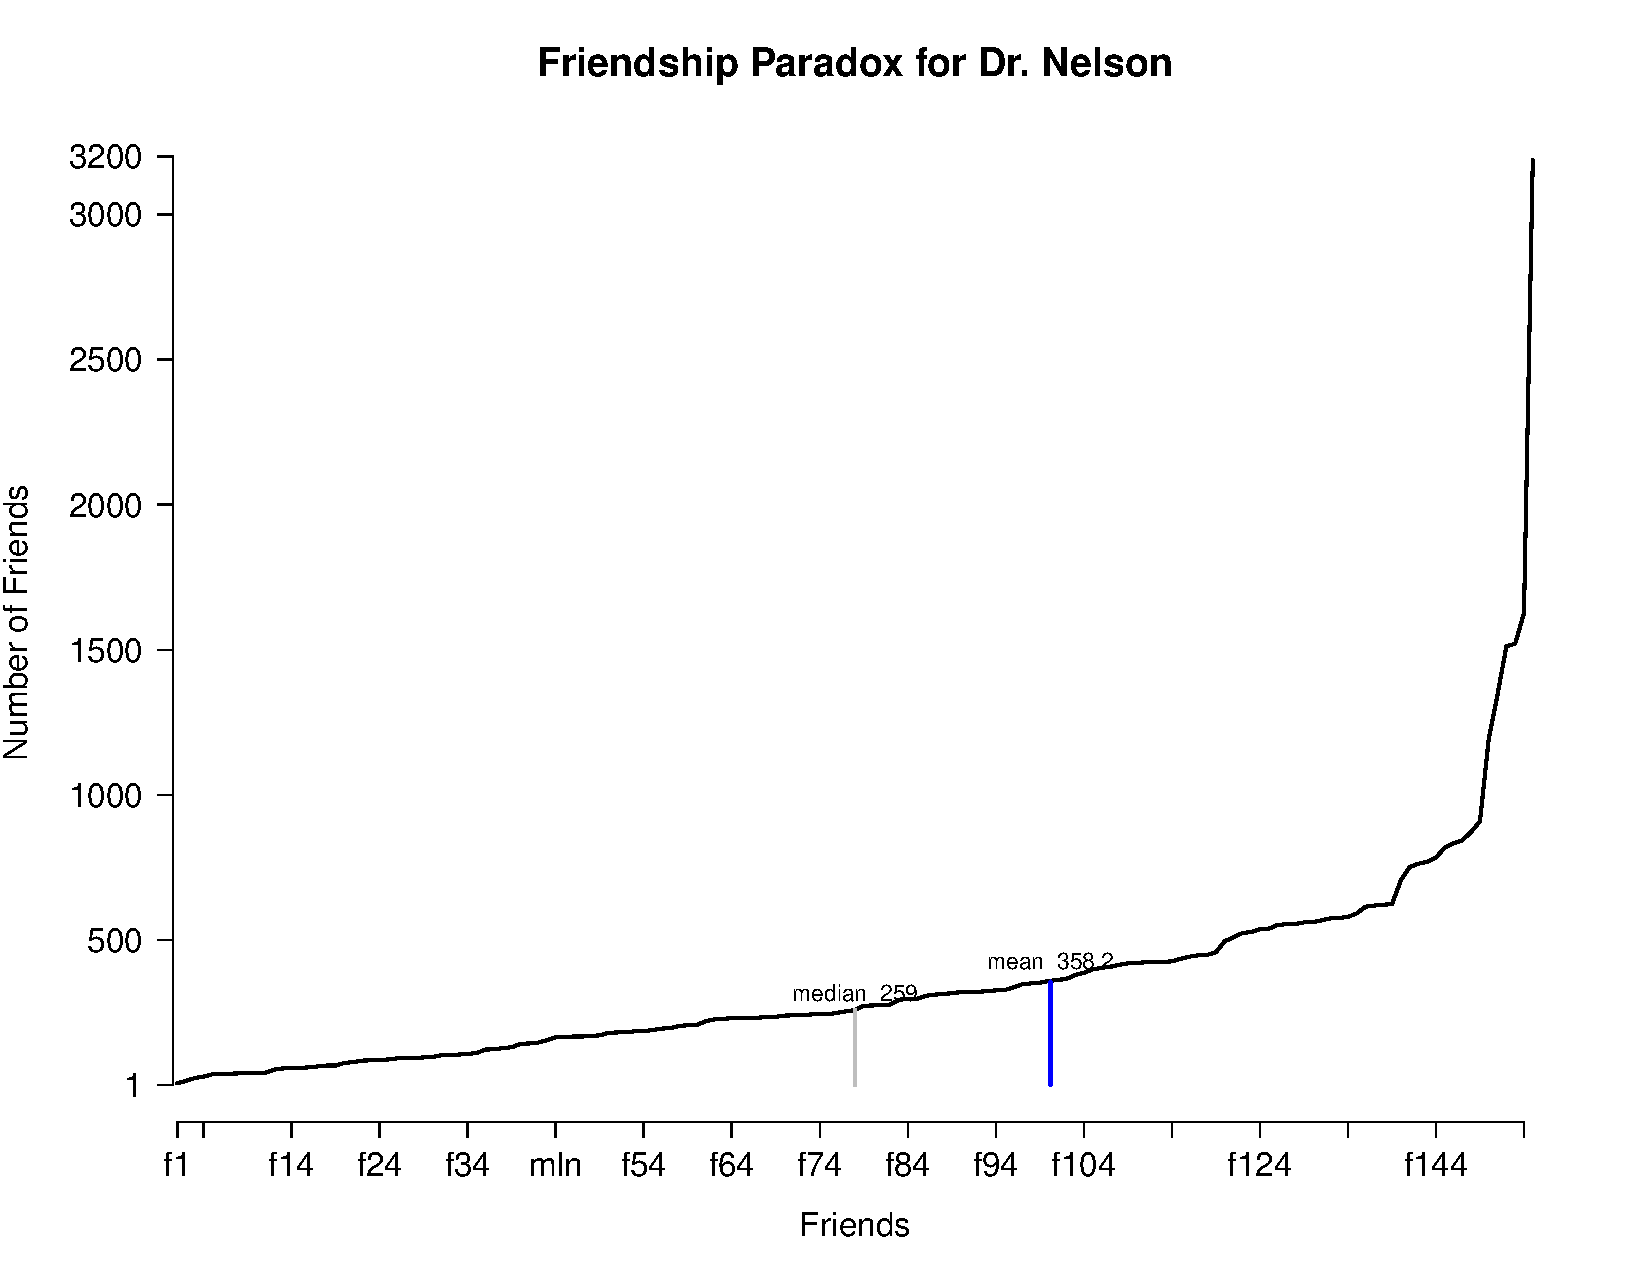
\includegraphics[scale=.5]{images/facebook-paradox.pdf}
\caption*{\scriptsize The data was sorted by \textbf{Number-of-Friends} field (see Table \ref{tab:table1}), the graph shows characteristics of a power-law distribution. The \textbf{Number-of-Friends} corresponding to $mln$ is \textcolor{red}{165} and $mln$ is positioned at the left side of the median \textcolor{red}{259}.  Thus, the friendship paradox holds true for $mln$ Facebook account.}
\end{figure}
\newpage
The mean, standard deviation, and median were computed using R. The file $<facebook.R>$ is the script that makes the computation and graph plotting. The file is attached to this document. Following is the calculation for the number of friends that $mln$ friends has:\\
\begin{itemize}
	\item Mean: \textcolor{red}{358.2}\
	\item $\sigma$: \textcolor{red}{259}
	\item Median: \textcolor{red}{370.7}
\end{itemize}
$\sigma$ has a high value. It is skewed due to the magnitude of the last 5 friends. See Table \ref{tab:table1}. However, even if we were to disregard this data,  $mln$'s Number of Friends are so far left from the mean and the median that the friendship paradox holds true for $mln$ Facebook account, in which his friends have more friends than he.
\end{homeworkProblem}

%----------------------------------------------------------------------------------------
%	Problem 2
%----------------------------------------------------------------------------------------
\newpage
\begin{homeworkProblem}
\vspace*{10pt} % Question
Determine if the friendship paradox holds for your Twitter account. Since Twitter is a directed graph, use \enquote{followers} as value you measure (i.e., \enquote{do your followers have more followers than you?}).\\

Generate the same graph as in question \#1, and calculate the same mean, standard deviation, and median values.\\

For the Twitter 1.1 API to help gather this data, see:\\

\url{https://dev.twitter.com/docs/api/1.1/get/followers/list}\\

If you do not have followers on Twitter (or don't have more than 50), then use my twitter account \enquote{phonedude\_mln}.

\subsection{2.1 Approach}

\textbf{EXTRACTING DATA}\\

My sister's Twitter account was employed to test if the paradox holds. A REST Twitter API \cite{api} $cURL$ command was used to execute the request:\\

\begin{verbatim}
 curl --get 'https://api.twitter.com/1.1/followers/list.json' --data
     'amp%3Binclude_user_entities=false&amp%3Bscreen_name=
     roselenavargas&amp%3Bskip_status=true&cursor=-1' 
     --header 'Authorization: OAuth oauth_consumer_key="L9IMyConSuMerKeyT1MC",
      oauth_nonce="33b5ab398f8145ac453017896ebe99a1",      
      oauth_signature="IQgpTL2PBvHzeu%2BKa7veW7EIxrw%3D", oauth_signature_method="HMAC-SHA1",
      oauth_timestamp="1456395318", oauth_token="412664119-
      YJ5IeQTheAuThoRizaTionToken", oauth_version="1.0"' --verbose > twitter
\end{verbatim}

The result was redirected to a file $<twitter>$. Since the result is a JSON object, the original approach was to utilize a Python library, such as $pickel$ or $json$ to create a structure to iterate and extract its data. Both approaches came empty, in which the number of followers extracted was less than in the data structure. This most likely was due to some type of encoding problem in the file. However, to move forward a third approach proved to be effective: the use of $regex$.\\

$<GetFollowers.py>$ is the Python program that helped extract the information needed to make the proof. The heart of the code is in line 25:

\lstinputlisting[language=Python,
                 style=mybox, 
                 captionpos=t,
                 caption={GetFollowers.py},
                 label=listing:Grep,
				 linerange={24-29},
				 firstnumber=24                 
                 ]
{../GetFollowers.py}

An iterable object was formed with the regular expression \texttt{`\textbackslash "followers\_count\textbackslash ":\textbackslash d+'}, extracting followers\_count amounts. Finally, my sister's information along her followers was placed in file $<twitter_paradox.dat>$. Table \ref{tab:table2} shows the data set result.

\subsection{2.2 Solution}
\begin{figure}[!h]
\caption{Sister's Twitter Followers Graph}\label{fig:2}
\center
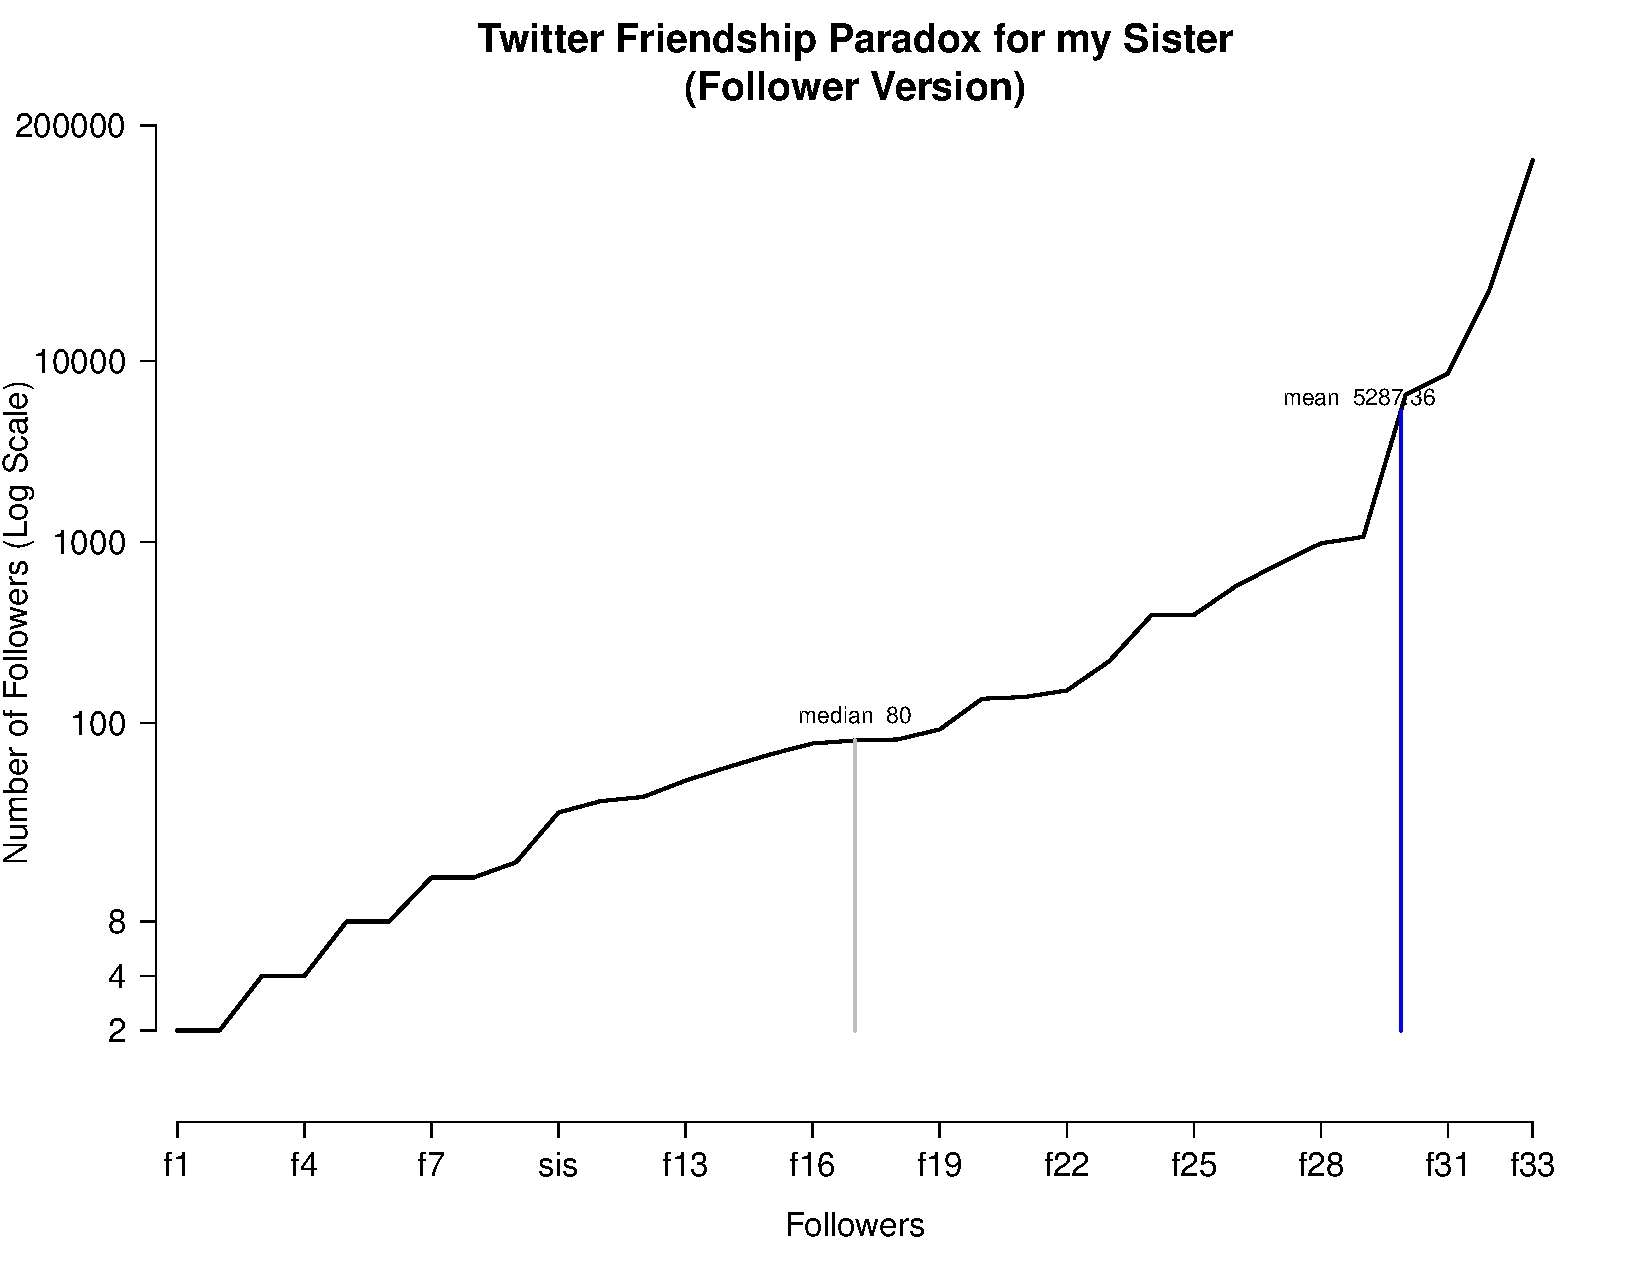
\includegraphics[scale=.5]{images/twitter-paradox.pdf}
\caption*{\scriptsize The data was sorted by \textbf{Number-of-Friends}, the graph shows characteristics of a power-law distribution. The \textbf{Number-of-Friends} corresponding to $sis$ is \textcolor{red}{32} (see Table \ref{tab:table2}). Since $my\ sister$ on the x-axis is positioned at the left side of the median \textcolor{red}{259} and the mean  \textcolor{red}{5287}, then the friendship paradox holds for my sister Twitter account, in which her friends have more followers than she.}
\end{figure}
The mean, standard deviation, and median were computed using R. The file $<twitter.R>$ is the script that makes the computation and graph plotting. The file is attached to this document. Following is the calculation for the number of friends that my sister's friends have:\\
\begin{itemize}
	\item Mean: \textcolor{red}{5,287.35}\
	\item $\sigma$: \textcolor{red}{22,623}
	\item Median: \textcolor{red}{80}
\end{itemize}
\end{homeworkProblem}


%----------------------------------------------------------------------------------------
%	Problem 3 Extra Credit 3 Points
%----------------------------------------------------------------------------------------
\newpage
\begin{homeworkProblem}[Problem 3 Extra Credit]
Repeat question \#1, but with your LinkedIn profile.
\subsection{3.1 Approach}
All the connections from my wife's LinkedIn account were downloaded in file $<source.txt>$. I couldn't cross reference the internal connection ID with their public ID, so a manual computation on the number of connections were employed to get the data.

\subsection{3.1 Solution}

\begin{figure}[!h]
\caption{Wife Linkedin Connection Graph}\label{fig:3}
\center
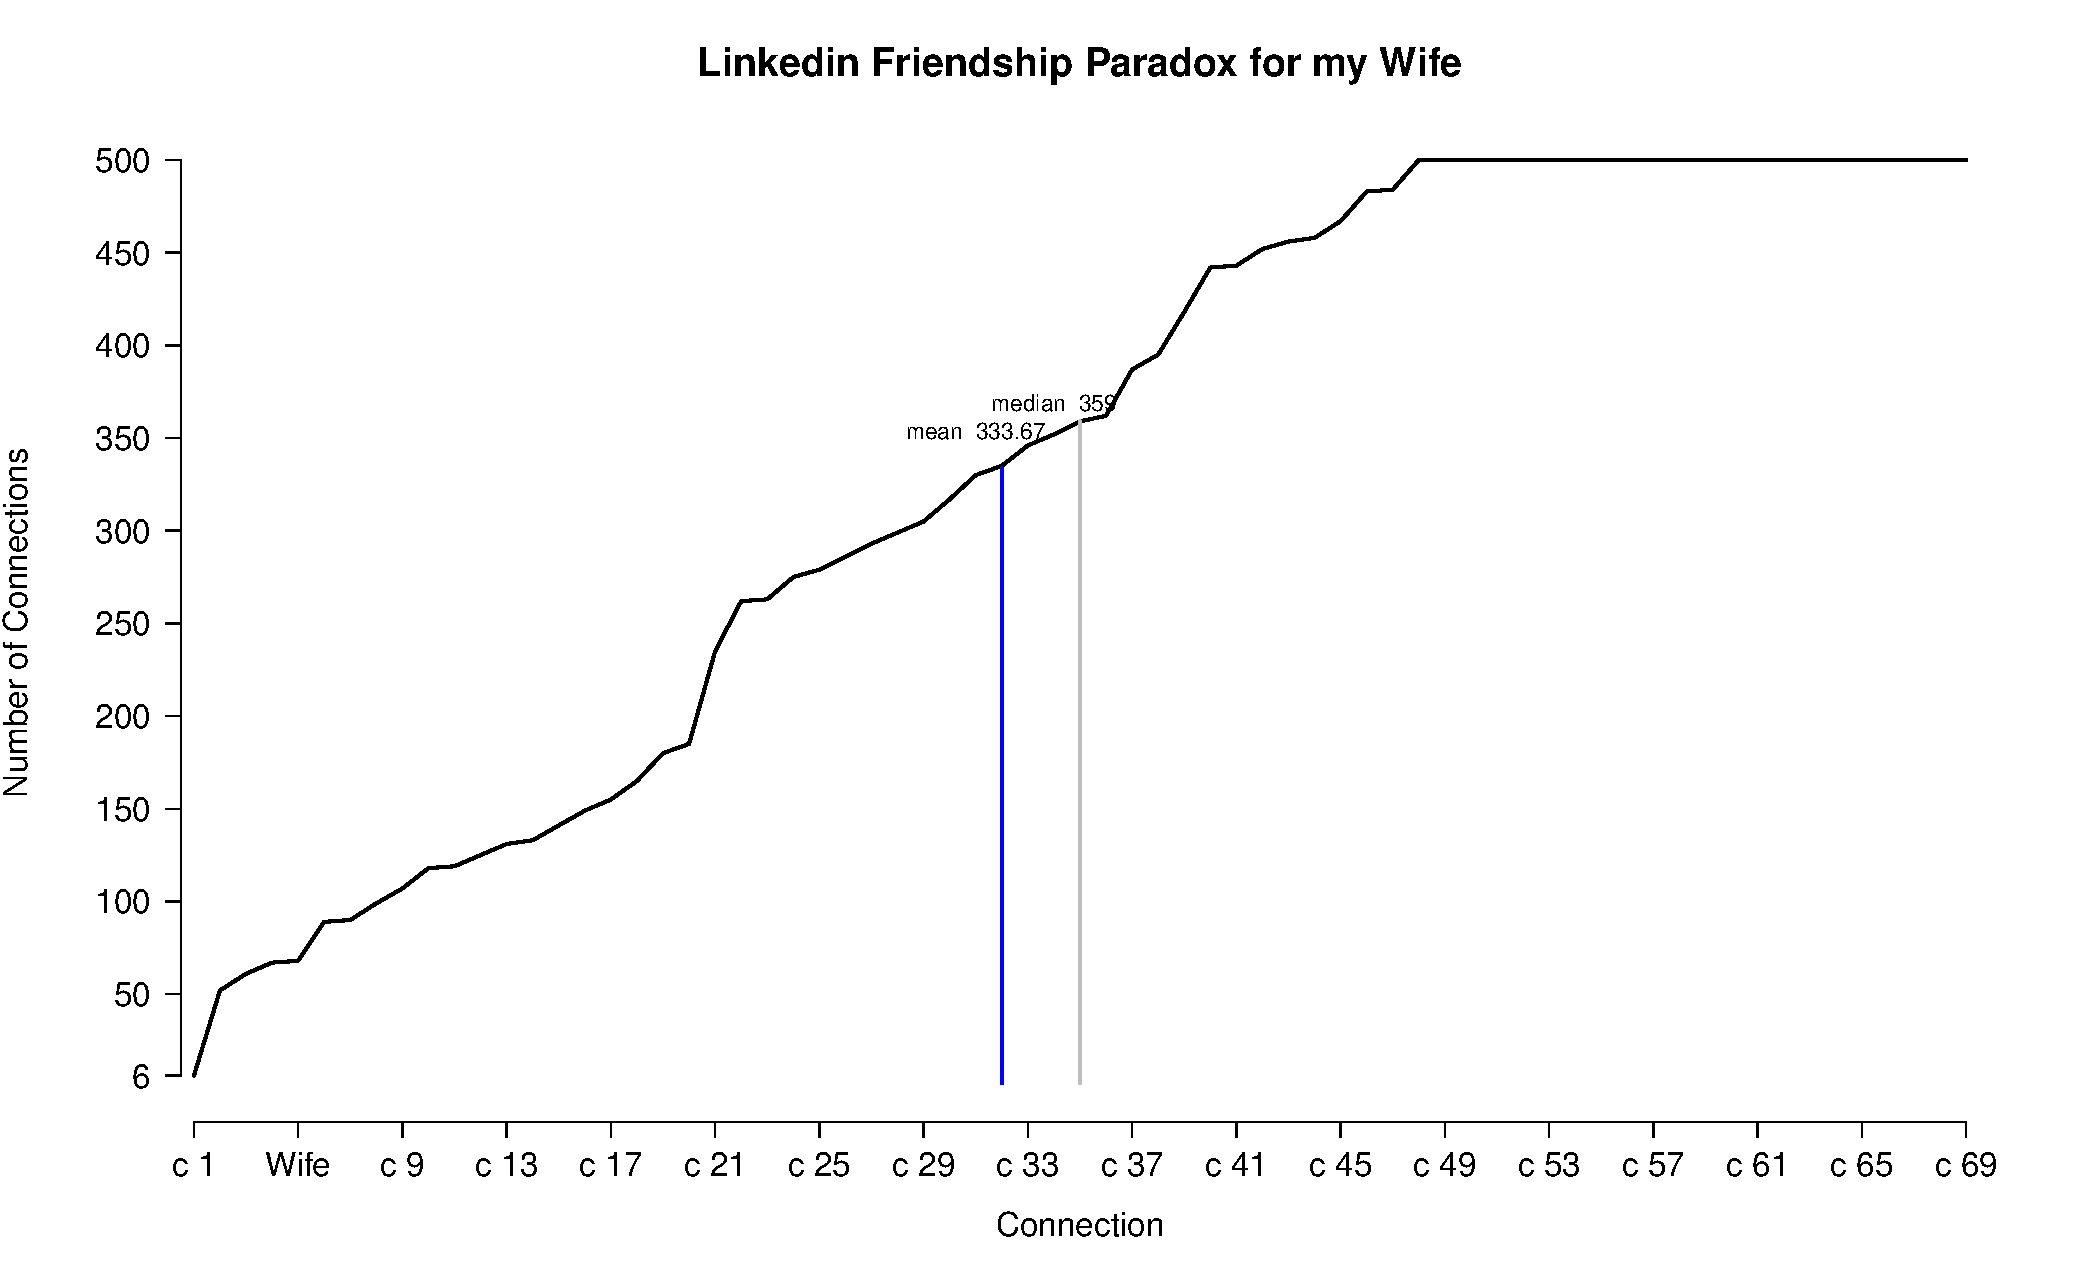
\includegraphics[scale=.45]{images/linkedin-paradox.pdf}
\caption*{\scriptsize The data was sorted by \textbf{Connection Count}. The \textbf{Connection Count} corresponding to $Wife$ is \textcolor{red}{68} (see Table \ref{tab:table3}) and $my\ wife$ is positioned at the left side of the median \textcolor{red}{359}. Then, the friendship paradox holds for my wife's Linkedin account in which her connections have  more connections than her.}
\end{figure}

The mean, standard deviation, and median was computed using R. The file $<linkedin.R>$ is the script that makes the computation and graph plotting. The file is attached to this document. Below the calculation results:\\
\begin{itemize}
	\item Mean: \textcolor{red}{333.67}\
	\item $\sigma$: \textcolor{red}{163.2}
	\item Median: \textcolor{red}{359}
\end{itemize}

\end{homeworkProblem}

%----------------------------------------------------------------------------------------
%	Problem 4 Extra Credit 1 Point
%----------------------------------------------------------------------------------------
\newpage
\begin{homeworkProblem}[Problem 3 Extra Credit]
Repeat question \#2, but change \enquote{followers} to {following}?  In other words, are the people I am following following more people?
\subsection{4.1 Approach}
The same approach as in 2.1 was followed. The only difference was that instead of using \textbf{follower\_count} as in the $regex$ filter, we used \textbf{friends\_count} which points to the number of particular person may be following. See listing below:

\lstinputlisting[language=Python,
                 style=mybox, 
                 captionpos=t,
                 caption={GetFollowing.py},
                 label=listing:Grep,
				 linerange={24-28},
				 firstnumber=24                 
                 ]
{../GetFollowing.py}

\subsection{4.1 Solution}

\begin{figure}[!h]
\caption{Sister's Twitter Following Friends Graph}\label{fig:4}
\center
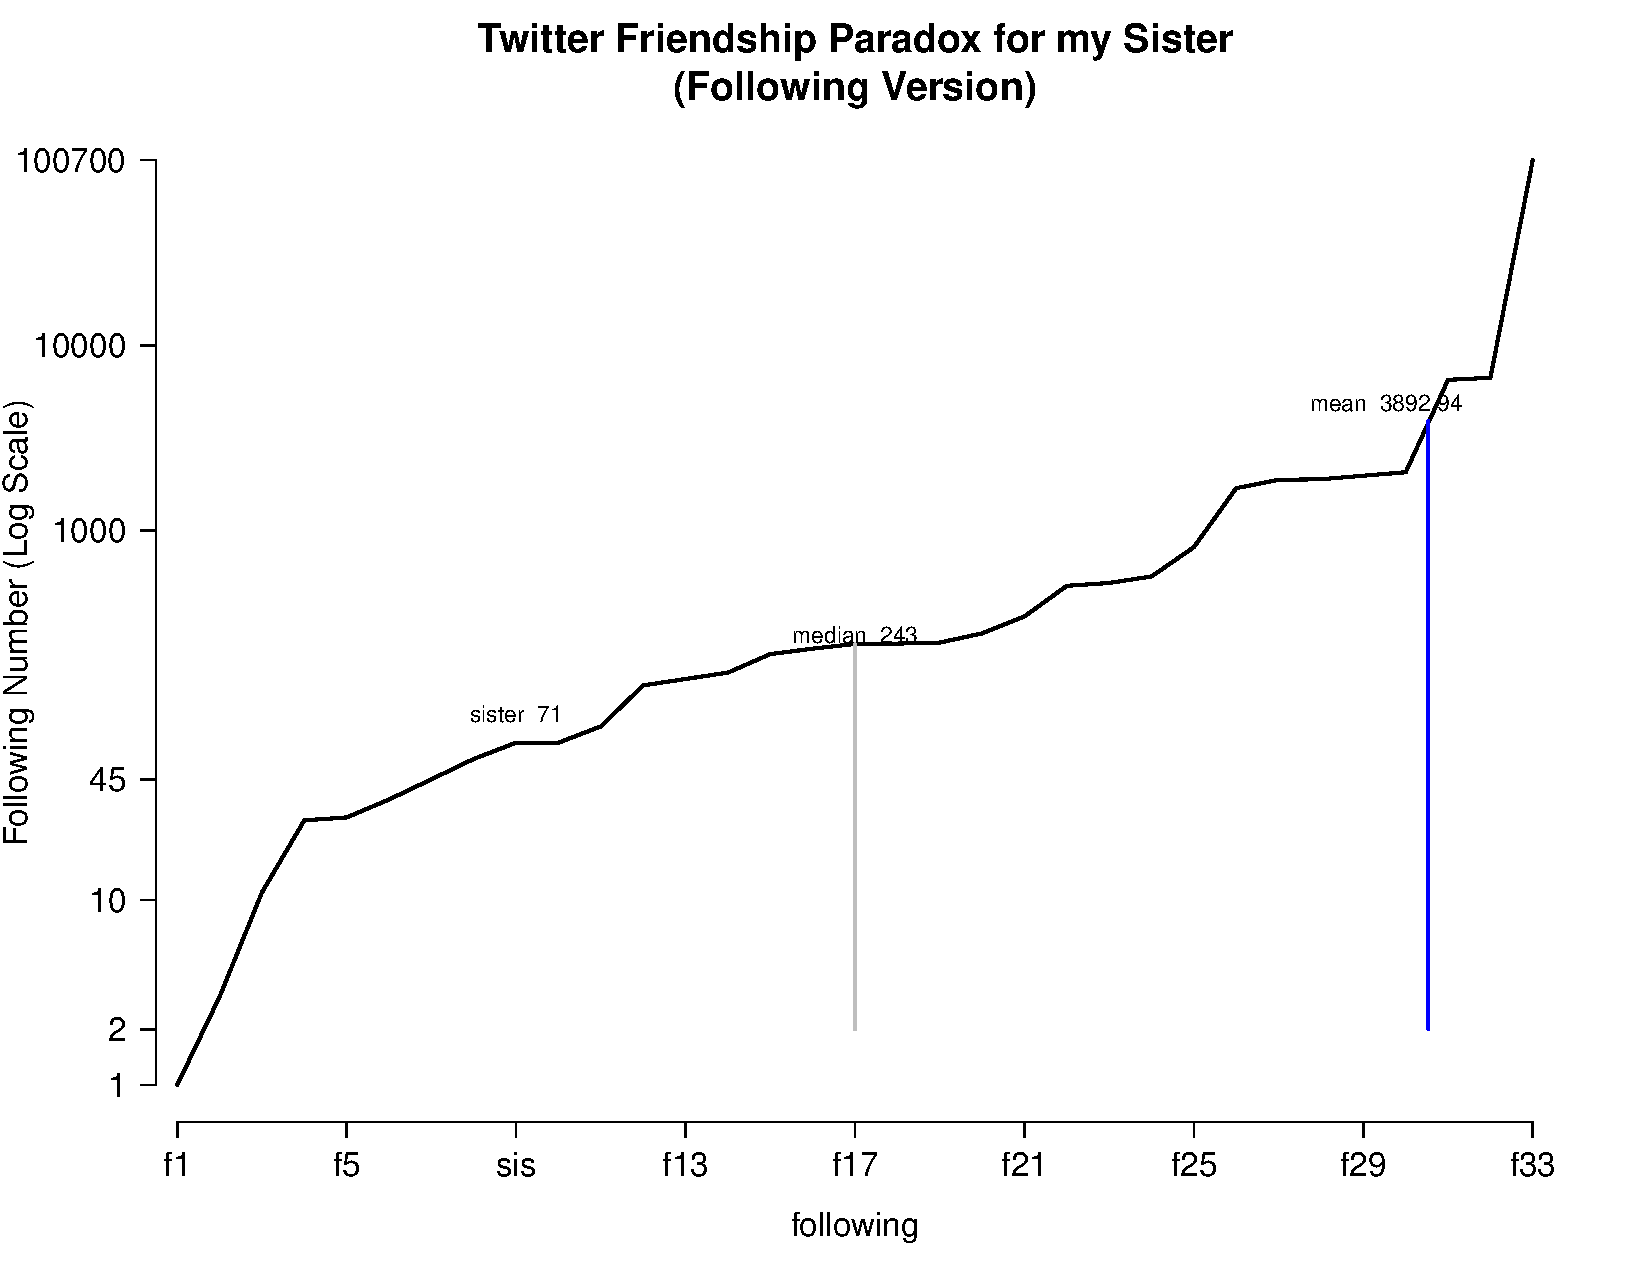
\includegraphics[scale=.5]{images/twitter-paradox2.pdf}
\caption*{\scriptsize Plotting the data sorted by \textbf{Number-Following}, the graph shows characteristics of a power-law distribution. The \textbf{Number-Following} corresponding to $sis$ is \textcolor{red}{71} and $my\ sister$ is position at the left side of the median \textcolor{red}{243}. Then, the friendship paradox holds for my sister Twitter account in which her friends are following more people than she.}
\end{figure}

The mean, standard deviation, and median were computed using R. The file $<twitter2.R>$ is the script that makes the computation and graph plotting. The file is attached to this document. Following is the calculation for the number of friends that my sister's friends have:\\
\begin{itemize}
	\item Mean: \textcolor{red}{3,892.94}\
	\item $\sigma$: \textcolor{red}{17,449}
	\item Median: \textcolor{red}{243}
\end{itemize}

\end{homeworkProblem}

%----------------------------------------------------------------------------------------
%	Tables
%----------------------------------------------------------------------------------------
\import{./}{tables.tex}
%----------------------------------------------------------------------------------------
%	Bibliography
%----------------------------------------------------------------------------------------
\newpage
\begin{thebibliography}{9}
%\bibitem{Lutz} 
%Lutz, Mark (2013). List and Dictionaries. \textit{Learning Python} (5th ed.). (pp. %262-263). Sebastopol, CA: O'Reilly Media.
%
\bibitem{api}
Twitter API. (n.d.) Retrieved February 24, 2016, from 
\url{https://dev.twitter.com/docs/api/1.1/get/followers/list}

%\bibitem{web-size}
%Daily Estimate Size of the World Wide Web. (n.d.) Retrieve February 17, 2015, from \url{http://www.worldwidewebsize.com/}

%\bibitem{google}
%Football Google Search. (n.d.) Retrieve February 17, 2015, from \url{http://www.google.com/?gws_rd=ssl#q=football/}
\end{thebibliography}
\end{document}
